% use paper, or submit
% use 10pt, 11pt or 12pt
% nopagenum removes the page numbers (final conference PDF paper)

%\documentclass[preprint, paper,11pt]{AAS}	% for preprint proceedings
\documentclass[paper,11pt]{AAS}		% for final proceedings (20-page limit)
%\documentclass[paper,12pt]{AAS}		% for final proceedings (20-page limit)
%\documentclass[paper,10pt]{AAS}		% for final proceedings (20-page limit)
%\documentclass[cover, article,11pt]{AAS}		% for journal paper version
%\documentclass[submit]{AAS}					% to submit to JAS

\usepackage{bm}
\usepackage{amsmath}
\usepackage{subfigure}
%\usepackage[notref,notcite]{showkeys}  % use this to temporarily show labels
\usepackage[colorlinks=true, pdfstartview=FitV, linkcolor= black, citecolor= black, urlcolor= black]{hyperref}
\usepackage{overcite}


\usepackage{color}
\usepackage[normalem]{ulem} % added this to enable sout for strike outs
\usepackage{float}



\definecolor{RED}{rgb}{1,0,0} 
\definecolor{BLUE}{rgb}{0,0,1} 
\definecolor{GREEN}{rgb}{0,0,1} 
\newcommand{\EditHPS}[1]{{\color{red} #1}}
\newcommand{\EditHPSd}[1]{{\color{red} \sout{ #1}}}
\newcommand{\EditEH}[1]{{\color{blue} #1}}
\newcommand{\EditEHd}[1]{{\color{blue} \sout{ #1}}}


\PaperNumber{18-078}
\CoverFigure{Figures/test} % Optional:  provide the path to the cover figure
\Conference{AAS Guidance, Navigation and Control Conference}
\ConferenceLocation{Breckenridge, Colorado}
\ConferenceDate{August 18--21, 2008}
% The following macros are used for the simulated journal article mode
\JournalName{Journal of the Astronautical Sciences}
\JournalIssue{Vol.~XX, No.~XX, XX--XX, XXXX, Pages XXX-XXX}
\JournalAuthors{Schaub}		% simulated article, authors in header
\JournalTitle{abcd}			% simulated article, brief title in header

\graphicspath{{../figs/} }


\begin{document}


\title{Towards Reinforcement Learning Techniques for Spacecraft Autonomy}

\author{Andrew Harris\thanks{Research Assistant, Ann and H.J. Smead Department of Aerospace Engineering Sciences, Graduate 
Student, University of Colorado Boulder, Boulder,
		CO, 80309 USA.},
		Hanspeter Schaub\thanks{Glenn L. Murphy Professor of Engineering, Department of Aerospace Engineering Sciences, 
			University of Colorado, 431 UCB, Colorado Center for Astrodynamics Research, Boulder, CO 80309-0431,  
		\href{mailto:hanspeter.schaub@colorado.edu}{hanspeter.schaub@colorado.edu}}
}


\maketitle{} 		


\begin{abstract}
Machine learning techniques present one class of strategies for addressing the problem of on-board spacecraft autonomy. Deep-space exploration missions, by nature, must deal with considerable uncertainty in their mission operations, especially those that deal with hard-to-model dynamics such as   atmospheric density. These challenges have arisen in concert with the development of techniques for considering and acting under uncertainty in the artificial intelligence or machine learning realms. In this work, a strategy for re-formulating the on-board maneuver decision-making problem in a framework amicable to the application of probabilistic machine learning techniques is presented using aerobraking as a demonstrative problem. Advantages and caveats of the methodology are outlined, with conceptual issues for solution approaches outlined. A simplified implementation of the autonomous aerobraking problem within an autonomy framework is presented to provide a basis for future developments in the field.
\end{abstract}


\section{Introduction}

The high cost of space mission operations has motivated several space agencies to prioritize the development of ``autonomous'' spacecraft control techniques \cite{Pecheur2000}. Of particular note are on-board autonomy techniques, which serve to expand spacecraft capabilities in environments where ground contact is not possible. While these techniques offer considerable promise, concerns remain regarding a variety of factors surrounding their implementation, such as the cost of developing such systems and their tolerance for un-modeled behaviors\cite{Starek2016}. Many of these issues are addressed in other fields through the application of machine learning (ML) techniques, which can provide autonomous systems with the ability to learn from and adapt to their environments without human intervention. These techniques, coupled with high-fidelity simulation tools, are a potential avenue for reshaping the manner in which flight systems are developed and fielded. 

Some modern mission proposals rely heavily on the use of phenomena in the space environment to enhance mission utility. A prominent example is aerobraking--the use of drag forces about planetary atmospheres to reduce spacecraft velocities--which has been proposed as a 
low-fuel method for controlling spacecraft since the dawn of the space age. While aerobraking has achieved 
success in missions like the Mars Reconnaissance Orbiter and Mars Odyssey \cite{Long2008}, both missions experienced
long periods of sustained, high-tempo operations during aerobraking phases. These periods of sustained ground operations added overhead to the mission's cost and raised the risk of human error \cite{Spencer2007}. Due to these costs, NASA has made the 
development of on-board, autonomous aerobraking routines a priority \cite{Long2008}. Considerable efforts in this realm have 
already been undertaken in the form of NASA's Autonomous Aerobraking Development Software (AADS), a multi-component software package intended to address each aspect of the aerobraking problem \cite{Cianciolo2018}. While AADS has presented remarkable robustness in simulation, the recent experience of the Cassini end-of-life campaign demonstrates that even our best understanding of planetary atmospheres can be inaccurate to factors of two to three times \cite{Andrade2018}. The autonomous use of aerobraking techniques for the outer planets will require not just new materials and mission concepts, but also systems to autonomously identify and manage large variances in atmospheric dynamics.

\begin{figure}[h]
	\centering
	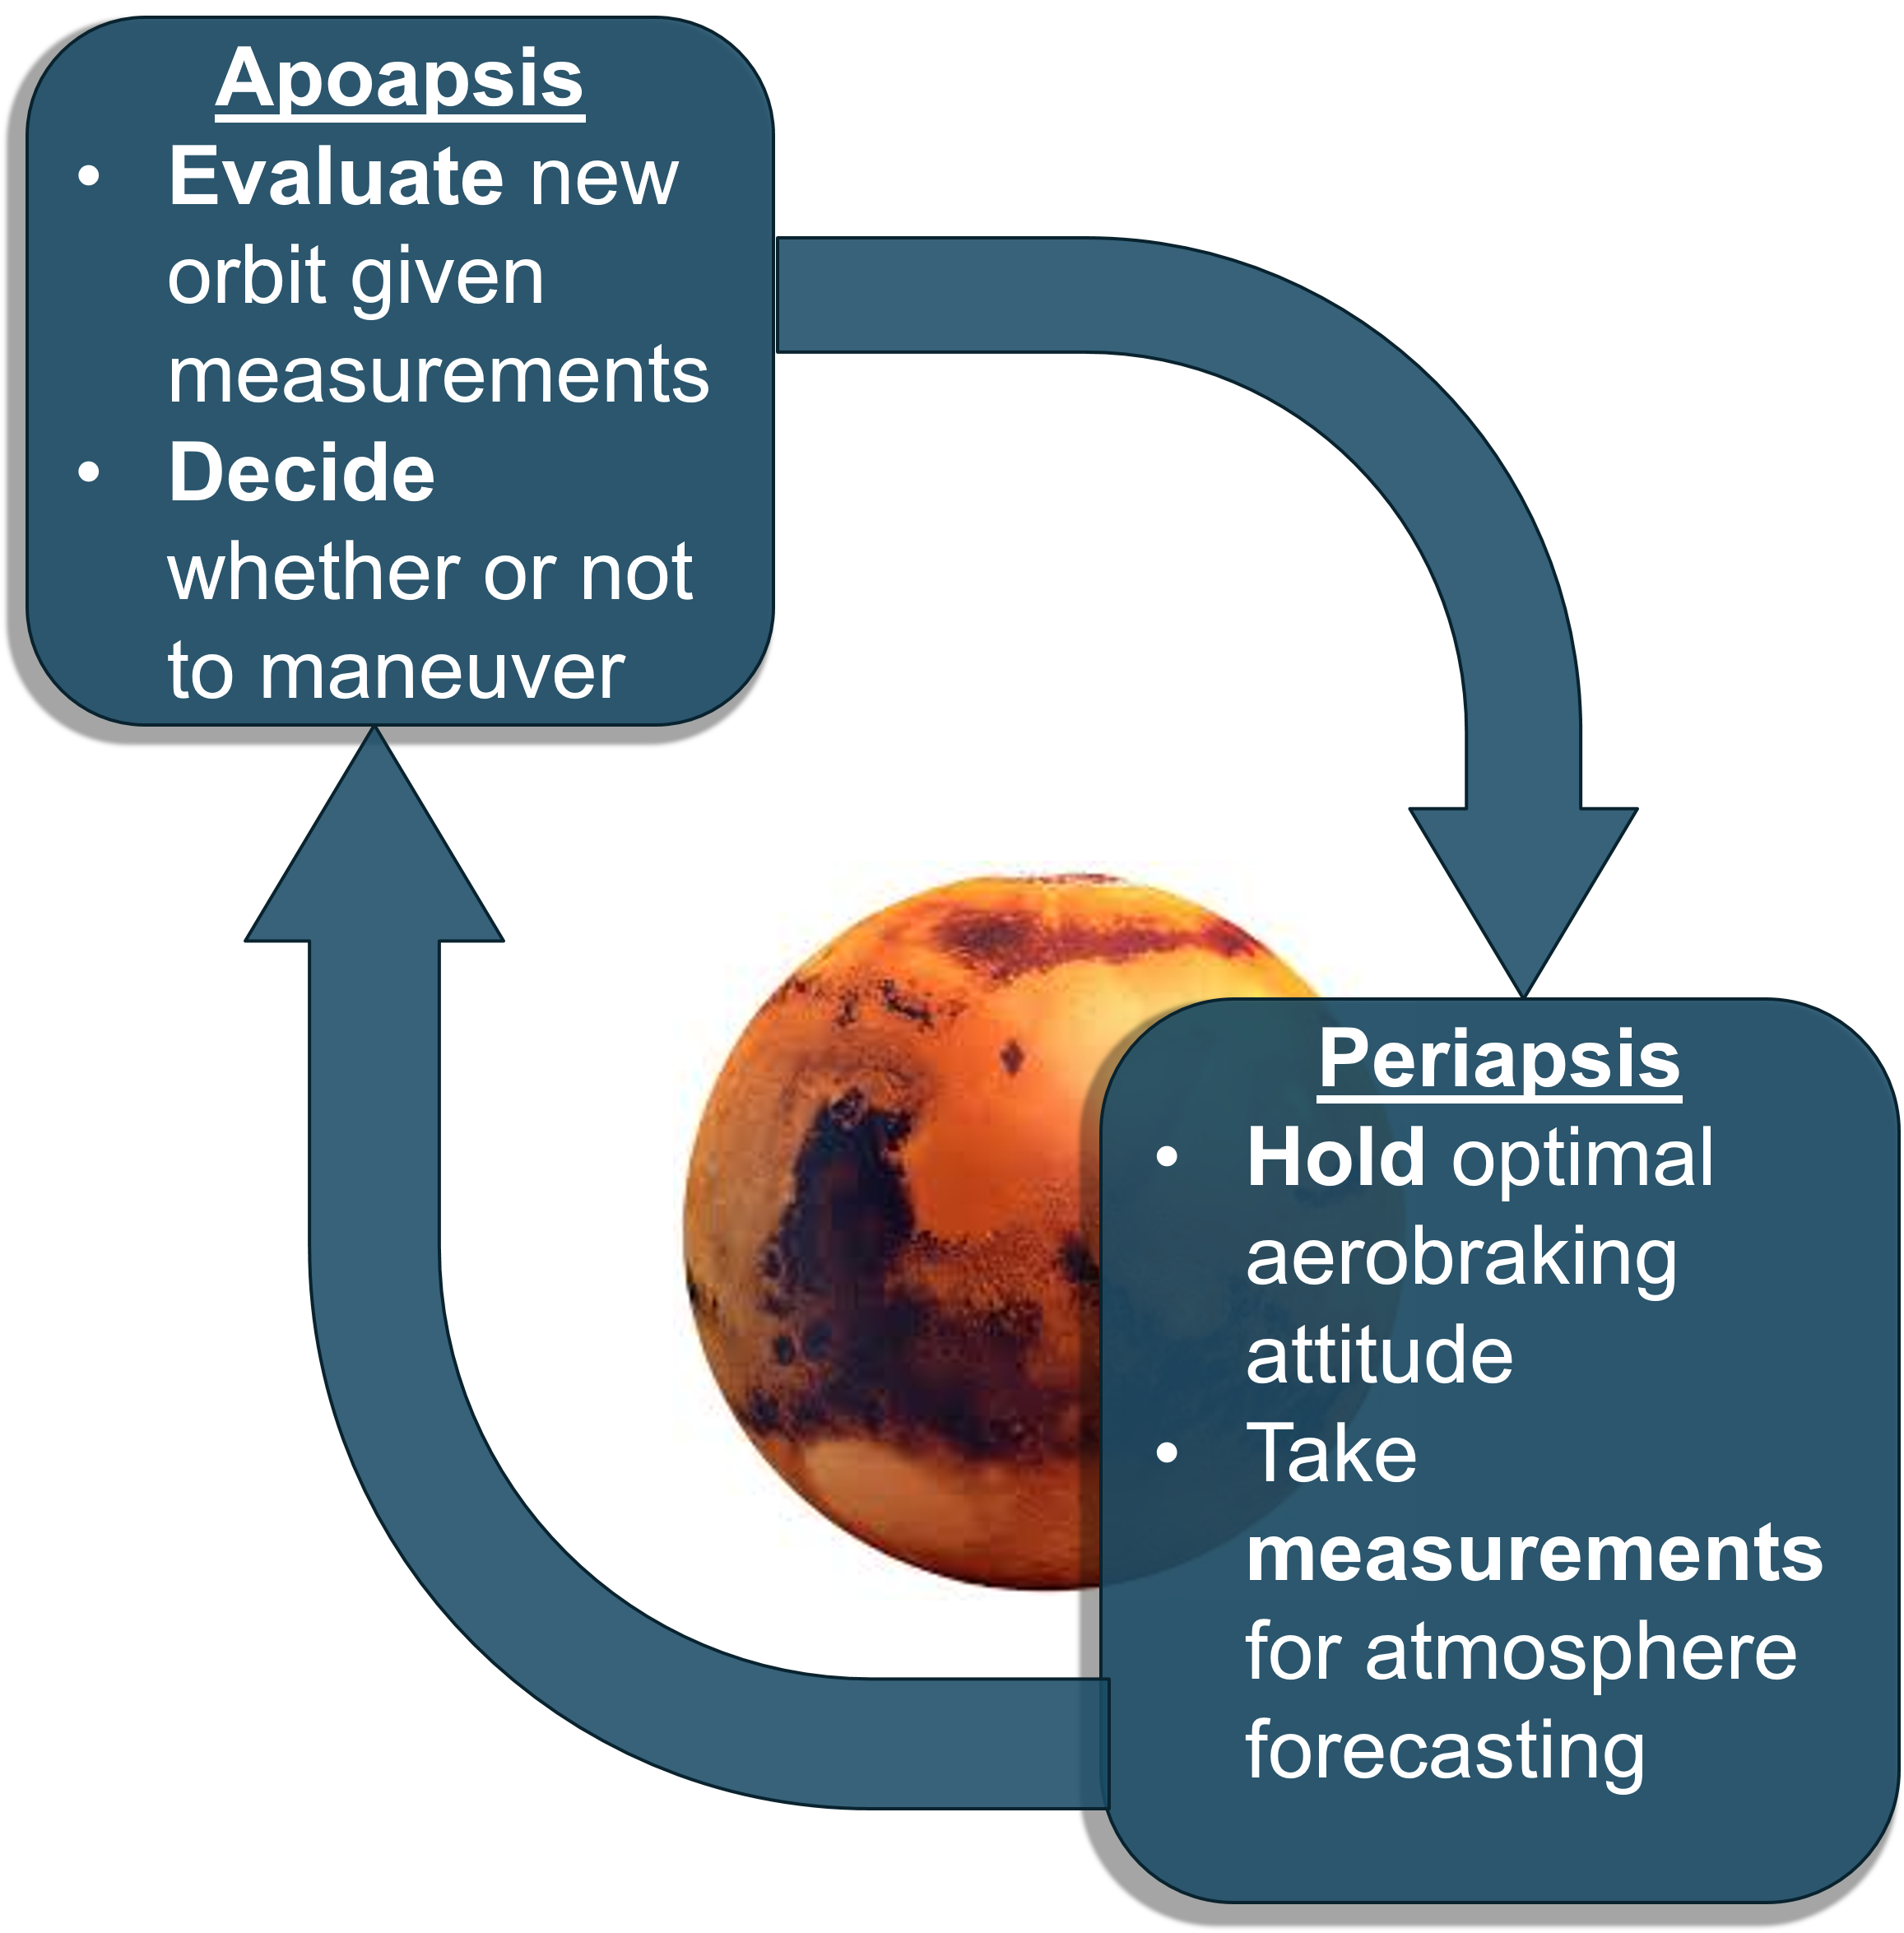
\includegraphics[width=2.5in]{aeroDecisionmaking.png}
	\caption{Graphical depiction of aspects of the autonomous aerobraking decision problem.}
	\label{fig:aerobrakingChoices}
\end{figure}

At the same time, there is considerable concern over the cost of developing and testing autonomous flight software systems. Frost \cite{Frost2010} outlines many of the issues facing the application of on-board spacecraft autonomy. He notes that the addition of autonomy increases the complexity and therefore cost of any given flight software system, which must be compensated for by some other benefit. This sentiment is echoed by others within the flight software community, for whom the verification and validation of complex, non-deterministic autonomy algorithms remains a concern and barrier to flight \cite{Pecheur2000}. 

Machine learning appears to offer solutions to both the task of adapting autonomous flight software systems to uncertain dynamics and to reducing life-cycle development costs for autonomous software development. By definition, machine learning techniques improve their performance through experience with the environment without the need for human intervention. Rather than carefully crafting rule-sets and databases by hand, future mission developers could leverage emerging high-fidelity astrodynamics software packages and off-the-shelf reinforcement learning techniques to address autonomy problems in a robust, adaptive manner. In this sense, machine learning strategies additionally provide a common framework for the consideration of problems in autonomy.

This work aims to identify promises and challenges of applying modern on-board reinforcement learning methods to astrodynamics problems. First, a brief introduction to reinforcement learning techniques for autonomy are presented, with a strategy for implementing these techniques and specific issues in astrodynamics addressed. Next, the problem of autonomous aerobraking is considered to demonstrate specific features and challenges of aerobraking as a representative problem for autonomy. Finally, the aerobraking problem is reformulated in a manner solvable by common reinforcement-learning techniques. 


\section{Reinforcement Learning Framework and Benefits}

Modern autonomy techniques frequently use so-called ``reinforcement-learning''(RL) approaches to address the problem of decision-making under uncertain or complex dynamics. These techniques facilitate the design of robust, flexible control schemes for  complex, non-linear or uncertain systems with relatively small design efforts. Additionally, they are readily extended to on-line techniques that can be used to 
incorporate real data. These factors make them attractive for general-purpose use in addressing on-board autonomy problems in astrodynamics.

Reinforcement learning techniques are usually considered in the context of Markov Decision Processes  (MDPs) or their less-tractable cousin, Partially-Observable Markov Decision Processes (POMDPs) \cite{Cassandra1997}. A POMDP is a four-tuple consisting of a set of states $S$, a set of actions $A$, a set of observations $O$, a set of rewards $R$, and mappings that relate these variables. A general POMDP is shown in Figure \ref{fig:classicalPOMDP}. The objective of reinforcement learning is to select a set of actions that maximizes the sum of rewards over the POMDP \cite{Sutton2012}. While there are many caveats involved in addressing POMDPs, they provide a convenient and compact framework for considering many inter-related aspects of autonomous decision-making problems.

\begin{figure}[!b]
	\centering
	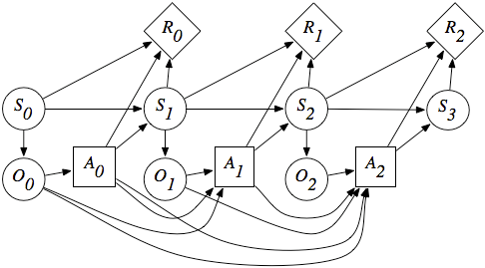
\includegraphics[width=2.5in]{classicalPOMDP.png}
	\caption{Bayesian network POMDP with states $s_i$, actions $A$, and rewards $R$. }
	\label{fig:classicalPOMDP}
\end{figure}

The theory of POMDPs is bolstered by the introduction of Bayesian networks. A Bayesian network compactly describes the relationships between stochastic variables by encoding them in a structure of nodes and edges, with transition probabilities governed by a set of model parameters denoted $\theta$. These parameters are themselves stochastic and can be estimated, allowing reinforcement learning techniques to improve their understanding of transition probabilities as they ``learn,'' thereby allowing them to adapt to uncertainty in underlying models on-line.  

The use of reinforcement learning to approximately solve POMDPs presents a convenient, compact, and holistic approach to designing autonomous decision-making algorithms. By incorporating probabilistic modeling from the ground up, properly implemented algorithms designed to address POMDPs provide more robust outcomes than other rule- or tree-based decision-making approaches. Importantly, reinforcement learning techniques do not generally require human designers to edit code beyond specification of problem dynamics or associated rewards, reducing the amount of code that must be directly handled or changed. 


\subsection{Implementation Concept of Operations}

Application of reinforcement learning techniques is typically considered in two phases: the ``training'' of a given algorithm on an environment, and the subsequent application of said algorithm to the environment (which may or may not include additional training). 

\begin{itemize}
	\item \textbf{Algorithm and System Definition:} First, designers must formulate a POMDP to represent the specific problem their algorithm is intended to address. Features of this model and the problem are used to identify the reward or penalty functions suitable to the problem. Given these features, a suitable reinforcement learning technique can be selected.
	\item \textbf{Model Training through Simulation:} Simulated data representing best-understood conditions for a problem-specific environment would be used to train the aforementioned algorithm to achieve desired performance.
	\item \textbf{Online Learning:} Resulting trained algorithms are implemented on the flight system. Real-world measurements are used to simultaneously refine system models and improve the utility of on-board decision-making without operator intervention.
\end{itemize}

First, mission designers specify relevant problem dynamics (such as atmospheric drag or multi-body gravity) and relevant features to reward or penalize (such as achieving a final orbital condition) by means of specifying a POMDP. These characteristics are then used to inform the selection of exploration strategies and learning techniques from the set of existing methodologies.

With the system model and learning algorithm specified, the training of said algorithm can begin. Training of a given algorithm typically requires a large number of exposures to specified training environments or scenarios, and is therefore non-trivially time consuming depending on environment complexity. For problems in astrodynamics, the time to train a given algorithm is especially time-consuming due to the computational complexity of evaluating orbital mechanics using high-fidelity simulated dynamics. Time-efficient training of ML-based control algorithms therefore requires the use of simulators that are both high-fidelity and high-performance---such as the C/C++-based Basilisk simulation framework\cite{Alcorn2016}---alongside algorithms that are efficient at utilizing data. It should be noted that, while training times are potentially long, these periods do not require human supervision, freeing highly-trained and expensive programmers to pursue other tasks.

Once trained, RL-based decision-making algorithms can be used statically, such that learned action policies are not changed in flight, or dynamically wherein the algorithm continues to fit its models for state values, state transition probabilities, and other learn-able parameters using real measurements. This represents an important trade off between roust control performance in the face of uncertain environmental dynamics and the potential performance improvements through on-line learning.

\subsection{Issues for Spacecraft Reinforcement Learning}

Astrodynamics problems present a set of unique challenges compared to typical reinforcement-learning applications, Here, we attempt to enumerate them alongside potential solutions from the machine-learning world.

\textbf{High-Dimensional Spaces:} Many approaches to machine learning rely on discrete state- and action-spaces, which are typically both easier and faster to solve using common reinforcement learning techniques. As mentioned previously, orbital mechanics are typically treated continuously with respect to state variables and are additionally chaotic with respect to those initial conditions, making them poor candidates for discretization. 

This has been a growing area of interest for decades, as virtually all dynamical systems involve continuous state-action spaces. Smart and Kaelbling \cite{Smart2000} demonstrate the use of the \verb|Hedger| algorithm to fit functions based on observed data using a locally-weighted regression technique. More conventional estimation techniques, like Kalman filters, have also been used extensively to estimate unknown model parameters for higher-level reinforcement learning controllers. This approach has been successfully applied to other complex aerospace systems, including decisionmaking and control for helicopter flight \cite{Abbeel2007}.

\textbf{Information Sparsity:} Reinforcement learning results are typically shown after thousands or even hundreds of thousands of training iterations to satisfy an underlying need to fully sample a given space. For comparison, the aerobraking campaign of the Mars Reconnaissance Orbiter lasted for four-hundred and forty-five orbits. 

These relatively short time-lines must be addressed in the development of learning-based autonomy algorithms for astrodynamics problems through the use of algorithms that use data ``efficiently.'' One manner in which this can be accomplished is the use of ``expert'' priors. For systems like aircraft flight \cite{Abbeel2007}, the actions taken by experts are used as a base for reinforcement learning algorithms to operate.

\textbf{Mission Risks and Lack of Repeatability:} Unlike ground-based systems, space missions do not have the luxury of low-cost failures. For the aerobraking problem, inaccurate decision-making could easily lead to loss of spacecraft functionality or end-of-life. Additionally, many missions are unique in their trajectory, mission objectives, and bus design, making them poor candidates for the kind of ``episodic'' learning many reinforcement learning algorithms address. 

These issues can be addressed through both efficient use of available data, the use of so-called ``expert'' prior data for training, and the intelligent application to data-rich missions. The management of large low-Earth orbit cubesat constellations, such as PlanetLabs' Dove constellation \cite{Foster2016}, could present one data-rich use for on-board reinforcement learning.

\section{Problem Description}
\label{sec:problemDisc}
Breaking ground on the application of reinforcement learning to on-board autonomy problems requires first setting up astrodynamics problems in a manner amicable to the application of even simple reinforcement learning algorithms. Here, the problem of autonomous aerobraking is considered as a representative case to demonstrate how problems might be fit into the POMDP framework used by reinforcement learning techniques.


\subsection{Simplified Aerobraking Problem}

The objective of our restricted aerobraking problem is to reduce the semimajor axis of a given spacecraft to a specified quantity by exploiting atmospheric drag while also avoiding high aerodynamic loads and  collisions with the planet. This is accomplished by conducting periodic maneuvers to adjust the altitude of periapsis; ideally, the spacecraft would conservatively place periapsis to avoid specified large atmospheric loading while at the same time substantially reducing its orbital energy. Additionally, a desired final ``drag-free'' orbit is specified with a given radius of apoapsis $r_a$ and radius of periapsis $r_p$. 

Generally, the orbit of a spacecraft about a massive body is governed by a second-order nonlinear ordinary differential 
equation \ref{eqn:gravEqn} \cite{Vallado2013}:

\begin{equation}
\ddot{\bm{r}} = \frac{\mu}{r^3} \bm{r} + \bm{a}_{\text{perturb}}
\label{eqn:gravEqn}
\end{equation}

To account for the presence of atmospheric drag, the time-dependent drag acceleration $a_D$ is computed by applying Equation 
\ref{eqn:dragEqn} \cite{Vallado2013} using the known ballistic coefficient for the spacecraft $\beta_D$, the spacecraft's velocity 
relative to the planet's atmosphere, and the local neutral atmospheric density $\rho$.  Note that because the drag force only acts in 
opposition to the spacecraft's velocity, it can only affect the shape and size of the planar components of the spacecraft's 
orbit; no inclination-changing maneuvers are possible under this simple drag model \cite{Sutton2008}.

\begin{equation}
\bm{a}_D = -\frac{1}{2} \beta_D \rho \bm{\dot{r}}^T\bm{\dot{r}}
\label{eqn:dragEqn}
\end{equation}

Uncertainty in the atmospheric neutral density $\rho$ over an aerobraking is a 
primary driver of aerobraking risk. While a number of highly complex atmospheric models exist for the planets, we simplify the 
problem by selecting a two-parameter exponential atmospheric model of the form:

\begin{equation}
\rho = \rho_0 e^{\frac{-h}{h_0}}
\label{eqn:expAtmo}
\end{equation}
where $\rho_0$ is the base planetary density (i.e., the density when $r=0$) and $h_0$ is the atmosphere's characteristic scale height. Other perturbation forces, such as SRP or n-body gravity, are not considered for simplicity.

With the considered dynamics established, it is necessary to quantify the actions able to be taken by a spacecraft during the aerobraking phase. As mentioned previously, the dominant controlled parameter in an aerobraking scenario is the periapsis altitude $r_p$. For spacecraft with impulsive thrusters, it is readily known that the optimal point in an orbit to raise or lower periapsis occurs at apoapsis. As such, the restricted problem addressed herein will consider a spacecraft only capable of maneuvering at apoapsis, with the assumption that periapsis has already been lowered into the atmosphere by a pre-aerobraking maneuver.

Finally, to introduce the problem of unobserved variables, it is assumed that the spacecraft position and velocity are determined by an on-board optical navigation system, but the density and scale height are not measured. 

\subsection{Discretization Approach}
\label{sec:discretization}
Most approaches to approximately solving POMDPs rely on the existence of discrete state, observation, and action spaces. While some approaches can work with continuous state variables, a more common approach is to discretize the continuous state space into an approximate discrete state space. For some problems, this is more tractable than others; for example, 2D robot maneuvering problems can often be represented using a discrete pair of coordinates. However, most astrodynamics problems require the use of multiple dimensions by nature. Compounding this issue is the fact that most astrodynamics problems are both large in terms of possible states and chaotic with respect to small variations in those states, requiring the use of a large number of discrete states to provide accurate modeling. This quickly causes even straightforward problems to encounter the ``curse of dimensionality,'' wherein the number of states to be explored grows exponentially and the problem becomes computationally intractable. 

The presented aerobraking problem represents a reasonable case for simplification, as the control objective requires us only to adjust the two planar parameters of an orbit that correspond to the radius of periapsis and the radius of apoapsis, which are found from the set of Keplerian elements by:
\begin{equation}
r_a = a (1+e)
\end{equation}
\begin{equation}
r_p = a (1-e)
\end{equation}
These parameters provide a convenient stand-in for the true semimajor axis and eccentricity, as they directly correspond to our assumed exponential atmospheric density model. Discretization of these variables is accomplished by ``binning'' the spacecraft radius of apoapsis and radius of periapsis into $n$ discrete bins. The selection of $n$ and the spacing of the bins creates many knock-on concerns, but the structure of the dynamics provides one guide. Because the assumed atmospheric model is exponential, it is reasonable to logarithmically distribute bins from a specified lower boundary to a specified upper position.

Next, the decision process is restricted to occur only at apoapsis, allowing us to consider the ``discrete'' transition of the radii of apoapsis and periapsis over each orbit. This approach is sensible due to the underlying 
nature of the control problem; burns to affect periapsis are most efficient when conducted at apoapsis. Applying this approach 
leads to a discrete-time system in orbits. An important caveat is that each time-step is not actually of constant length, as 
the period of an orbit is governed by its semi-major axis. However, this is a reasonable approximation under the assumption 
that the orbit (and therefore timing) is well-determined 
through optical navigation or other means.

In general, the variables $\rho_0$ and $h_0$, the surface density and scale height respectively, vary with time, solar flux, 
geomagnetic variation, and other complex phenomena. While complex, high-fidelity models of atmospheric variation are publicly 
available, this initial analysis assumes that $\rho_0$ and $h_0$ are normally distributed about their reference values and 
remain constant over each atmospheric pass.

For the purposes of this work, the spacecraft radii of apoapsis and periapsis 
were selected as the state variables to be controlled. In a similar manner, the space of actions taken by the spacecraft 
must be discretized.
The action space was discretized into three simple actions: 
doing nothing (Action 1), raising the continuous radius of periapsis by 5\% (Action 2), or lowering the continuous radius of periapsis by 5\% (Action 3). These broadly capture the affect of burns at small unit burns at apoapsis. 

Under these discretizations, a Bayesian network can be constructed to represent the system dynamics. The designed network is shown in Figure \ref{fig:designedBN}. 
\begin{figure}[h]
	\centering
	\includegraphics[width=2.0in]{please_god}
	\caption{POMDP for the approximated aerobraking problem which relates the current states $s$ with the next-time states $s'$.}
	\label{fig:designedBN}
\end{figure}
This network defines the relationships between $r_a$, $r_p$, $\rho$, and the selected apoapsis burn $a$ and how they relate to the states at the next time $k+1$. 

Finally, the discretized problem is restricted in time to a discrete number of orbits $n$, which simplifies the learning process and reflects real pressures to conduct aero-assisted maneuvers in finite time. This has the additional benefit of allowing training to occur over \textit{episodes}, where a single episode represents a reasonable initial condition the algorithm might encounter.

\subsection{Reward Function Definition}
Critical to the function of any reinforcement learning technique is the definition of a reward function or, 
inversely, a cost function. As stated previously, the objective of any reinforcement learning algorithm is to maximize the 
reward an agent receives over a specified time-span given a particular set of actions and states. If the reinforcement learning 
algorithm is effective and maximizes the earned value, the designer's problem is reduced to selecting an appropriate sets of 
rewards to drive the algorithm towards desired behavior.

In the case of the aerobraking problem, several sources or sinks of value present themselves. A summary of sources and sinks considered for the restricted problem are shown in Table \ref{table:aerobrakingRewards}. 

\begin{table}[h]
	\centering
	\caption{\label{table:aerobrakingRewards} Reward Sources/Sinks for the restricted aerobraking problem.}
	\begin{tabular}{c|c}
		Positive Reward & Negative Reward \\
		\hline
		Achieving specified $r_a$ & Maneuvering \\
		Achieving specified $r_p$ & Violating boundary $r_p$/$r_a$ \\
		 & Aerobraking phase length
	\end{tabular}
\end{table}

A snapshot of the presented reward function used for our scenario is shown in Figure \ref{fig:simRewardFunction}. Rewards are only provided when the spacecraft reaches a designated apoapsis or periapsis radius. Small costs are imposed for maneuvers, while a large cost is imposed for reaching the planet surface (i.e., mission failure). Additionally, there is a small penalty at each time to discourage ``waiting'' strategies as suggested by Sutton \cite{Sutton2012}. 

To demonstrate this concept, a sample reward function was generated for the described discretization approach with $n=30$ bins for both the radius of apoapsis and the radius of periapsis (c.f. Figure \ref{fig:simRewardFcn}). Features of the reward function include a quadratic cost for ``state error'' (the difference between the current and desired bins), a large reward for reaching the desired states, and large penalties for violating minimum boundaries for both the apoapsis and periapsis corresponding to aerodynamic load limits. 

\begin{figure}[H]
	\centering
	\includegraphics[width=3.0in]{20orbs500samps_reward}
	\caption{Sample reward function value versus binned apoapsis and periapsis with 30 bins.}
	\label{fig:simRewardFunction}
\end{figure}

\section{Sample Learning Methodology}
\label{sec:learningMethod}
This work uses a model-based value iteration algorithm to achieve a desired aerobraking trajectory outcome under variable atmospheric conditions. As such, a probabilistic model of the system dynamics must be learned alongside the value (and therefore action) functions. This is accomplished in the frequentist technique suggested by Sutton\cite{Sutton2012}:

\begin{equation}
T(s,a | s',a') = \frac{N(s, a \rightarrow s')}{N(s,a)}
\end{equation}
\begin{equation}
R(s,a) = \rho(s,a)/N(s,a)
\end{equation}
where $N(s, a \rightarrow s')$ represents the current count of transitions between the previous state and the current state, $N(s,a)$ represents  the number of counts of the previous state, and $\rho(s,a)$ represents the sum of rewards received in a given state. This represents among the simplest possible algorithms for an on-board system to ``learn'' system probabilities and thereby approximate true system dynamics, representing a worst-case learning problem wherein even two-body mechanics are not taught to the spacecraft. 

At the apoapsis of each orbit, the current $r_a$, $r_p$, and associated reward $r_k$ are provided to the learning algorithm. These are used to update the state-value function $Q$ by the \textit{Dyna} algorithm suggested by Sutton \cite{Sutton2012}:
\begin{equation}
Q(r_{a}, r_{p}, a) = R(r_{a}, r_{p}, a) + \gamma \sum_{r_a', r_p'} T(r_a', r_p' | r_a, r_p, a)\text{max}_a(Q(r_a', r_p', a'))
\end{equation}
In this sense, the algorithm attempts to tailor its learned value function to more closely match the ``true'' value function, and the  current control scheme to maximize value within the learned value function. Importantly, the sequential nature of these steps allows for them to be computed on-line, for example during aerobraking campaigns. In this manner, reinforcement-learning based control could autonomously adapt to changes in the underlying atmospheric model without operator intervention.

\section{Conclusions and Future Work}

Reinforcement learning represents the current state-of-the art in machine autonomy, but has found relatively little application towards on-board autonomy for astrodynamics use. The techniques and methodologies outlined in this work represent the first step towards the use of reinforcement learning to improve autonomous spacecraft performance and robustness to complex, un-modeled dynamics. Currently, the methodology outlined in Section \ref{sec:learningMethod} is being investigated to provide a baseline for future investigations using more suitable state and action-space representations. 

The aforementioned modeling and learning approach presents a credible method for improving the autonomy and performance of future aerobraking spacecraft. Comparisons between traditional rule-based aerobraking schemes, reinforcement-learned planning techniques using static training data, and techniques using on-line training methods will be compared on performance metrics like fuel use, aerobraking maneuver duration, and actual aerodynamic and thermal loads during aerobraking passes.

\bibliographystyle{AAS_publication}   % Number the references.
\bibliography{revisedFinal.bib}   % Use references.bib to resolve the labels.


\end{document}
